\documentclass[10pt]{beamer}

\usetheme{CambridgeUS}
\usepackage[english, russian]{babel}
\usepackage[utf8]{inputenc}
\usepackage{caption}
\usepackage{etoolbox}
\usepackage{multicol}
\usepackage{listings}
\usepackage{wasysym}
\usepackage{mathtools}
\DeclarePairedDelimiter\ceil{\lceil}{\rceil}
\DeclarePairedDelimiter\floor{\lfloor}{\rfloor}

\definecolor{mygreen}{rgb}{0,0.6,0}
\lstset{
  basicstyle=\ttfamily\footnotesize,        % the size of the fonts that are used for the code
  breaklines=true,                 % automatic line breaking only at whitespace
  captionpos=b,                    % sets the caption-position to bottom
  commentstyle=\color{mygreen},    % comment style
  keywordstyle=\color{blue},       % keyword style
  stringstyle=\color{red},     % string literal style
  showstringspaces=false,
  morekeywords={include, printf},
  texcl=true     %<---- added
}


\title[\href{https://goo.gl/NRgp8K}{https://goo.gl/NRgp8K} (Term 1)]{Графы. BFS. Планарность}
\author[Гусев Илья, Булгаков Илья]{Гусев Илья, Булгаков Илья}
\institute[МФТИ] 
{Московский физико-технический институт\\*}
\date{Москва, 2018}
\subject{Computer Science}

\begin{document}

\begin{frame}
  \titlepage
\end{frame}

\begin{frame}{Содержание}
\tableofcontents
\end{frame}

\subsection{Графы. BFS. Приложения}

\begin{frame}[fragile]{BFS. Поиск минимального цикла}
Как найти минимальный цикл в ориентированном невзвешенном графе?
    \begin{itemize}
        \item Запустим поиск в ширину из каждой вершины; 
        \item как только в процессе обхода мы пытаемся пойти из текущей вершины по какому-то ребру в уже посещённую вершину, то это означает, что мы нашли кратчайший цикл, и останавливаем обход в ширину; 
        \item среди всех таких найденных циклов (по одному от каждого запуска обхода) выбираем кратчайший.

    \end{itemize}
\end{frame}

\begin{frame}[fragile]{BFS. Проверка на двудольность}
Как определить, является ли граф двудольным?
    \begin{itemize}
        \item Произведём серию поисков в ширину. Т.е. будем запускать поиск в ширину из каждой непосещённой вершины. 
        \item Ту вершину, из которой мы начинаем идти, мы помещаем в первую долю. В процессе поиска в ширину, если мы идём в какую-то новую вершину, то мы помещаем её в долю, отличную от доли текущей вершину. Если же мы пытаемся пройти по ребру в вершину, которая уже посещена, то мы проверяем, чтобы эта вершина и текущая вершина находились в разных долях. В противном случае граф двудольным не является.
        \item По окончании работы алгоритма мы либо обнаружим, что граф не двудолен, либо найдём разбиение вершин графа на две доли.

    \end{itemize}
    
\end{frame}

\begin{frame}[fragile]{BFS. Поиск количества минимальных путей между вершинами}
Как найти количество различных кратчайших путей между заданными вершинами src и dst?
    \begin{itemize}
        \item Запускаем модифицированный BFS. Для каждой посещенной вершины храним длину минимального пути в нее и число уже найденных путей в нее.
        \item При каждом заходе в посещенную вершину обновляем ее "показатели". Если найден более короткий путь, то сбрасываем счетчики. Если путь длиннее - игнорируем его. Если путь такой же - увеличиваем счетчик числа путей.
    \end{itemize}
    
\end{frame}

\subsection{Планарные Графы}

\begin{frame}[fragile]{Планарный граф}
\textbf{Плоский граф} — это граф, нарисованный таким образом, что его ребра не пересекаются. 

Граф допускает \textbf{плоскую укладку}, если его можно нарисовать как плоский. 

Плоские графы называют \textbf{планарными}.
    
\end{frame}

\begin{frame}[fragile]{Пример планарного графа}
Граф является планарным, так как его можно нарисовать так, чтобы его ребра не пересекались
\begin{center}
    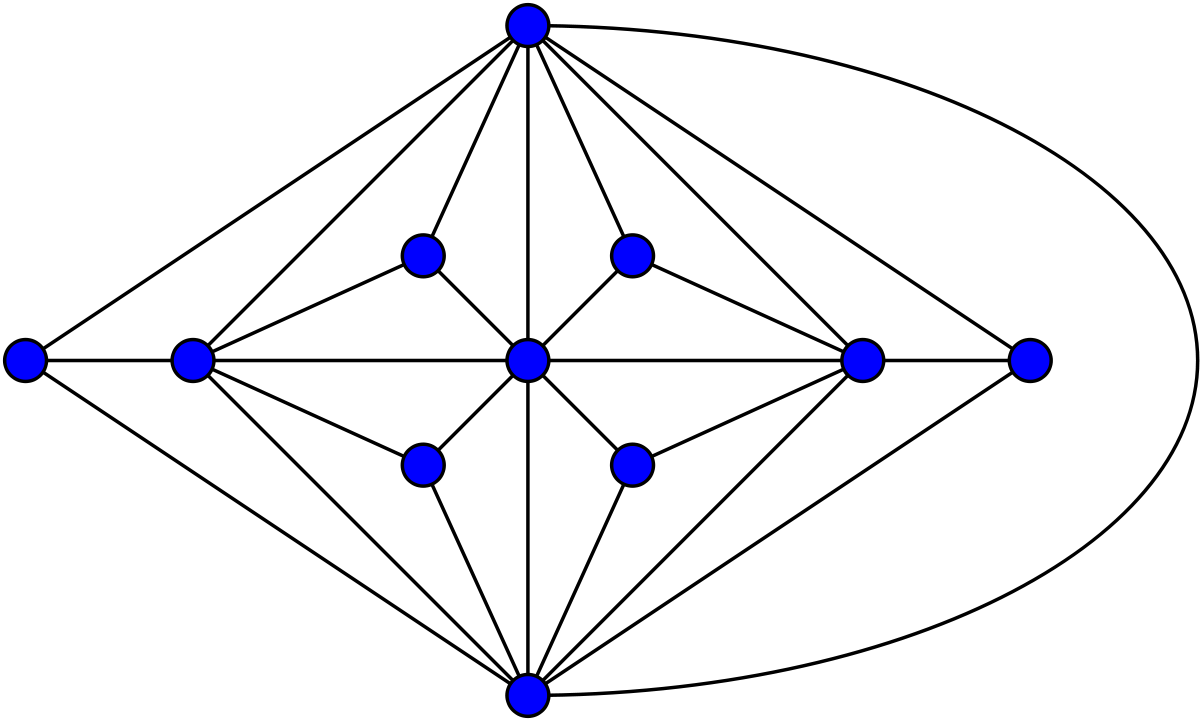
\includegraphics[width=8cm]{Term_2/Source/images/4_planar.png}
\end{center}
\end{frame}

\begin{frame}[fragile]{Пример непланарного графа}
Здесь показаны два непланарных графа: полный пятивершинник и полный двудольный граф. Для них есть специальные обозначения: K5 и K3,3 соответственно.
\begin{center}
    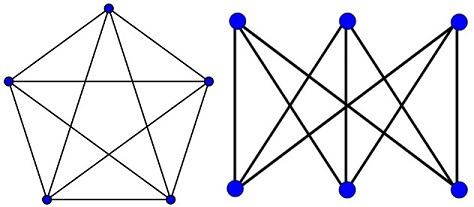
\includegraphics[width=10cm]{Term_2/Source/images/4_k33_k5.jpeg}
\end{center}
\end{frame}

\subsection{Задача о плоской укладке.}

\begin{frame}[fragile]{Задача о плоской укладке.}
Задача: Определить, является ли граф планарным, и, если да, то произвести его плоскую укладку.
    \begin{itemize}
        \item Теория. Есть теорема Понтрягина-Куратовского, которая утверждает: граф планарен тогда и только тогда, когда он не содержит подграфов, гомеоморфных К5 и К3,3. Представляет теоретический интерес.
        \item Практика. Есть алгоритмы, которые позволяют построить плоскую укладку, если она существует. Рассмотрим \textbf{гамма-алгоритм}.
    \end{itemize}
    
\end{frame}

\subsection{Гамма-алгоритм.}

\begin{frame}[fragile]{Гамма-алгоритм}
Гамма-алгоритм: построение плоской укладки.

Входные данные:
    \begin{itemize}
        \item Граф связный. Если граф несвязный, но рассматриваем каждую компоненту связности. (Повторение: как найти компоненту связности?)
        \item Граф имеет хотя бы один цикл. Если граф - дерево, то он планарен.
        \item Граф не имеет мостиков, т. е. ребер, после удаления которых граф распадается на две компонеты связности. Если мосты есть, они убираются и компоненты укладываются по очереди: каждая последующая укладывается на правильной грани.
    \end{itemize}
    
\end{frame}

\begin{frame}[fragile]{Гамма-алгоритм}
Гамма-алгоритм: формальное описание
    \begin{itemize}
        \item \textbf{Инициализация}: Выберем любой простой цикл C исходного графа G; изобразим его на плоскости в виде грани, которую примем за уже уложенную часть $G^{plane}$; сформируем сегменты $S_i$; если множество сегментов пусто, граф уложен
        \item \textbf{Шаг алгоритма}. Пока множество сегментов непусто:
        
            \begin{itemize}
                \item Для каждого сегмента S найти множество $\Gamma(S)$. Если существует сегмент S, для которого $|\Gamma(S)| = 0$, то граф не планарный, конец.
                \item Выбираем один из сегментов с минимальным числом вмещающих его граней.
                \item Выбираем одну из подходящих граней для выбранного сегмента. 
                \item В данном сегменте выбираем цепь между двумя контактными вершинами и укладываем ее в выбранной грани. Учтем изменения в структуре сегментов. Переход к новому шагу
            \end{itemize}
        \item \textbf{Завершение}. Построена плоская укладка $G^{plane}$ исходного графа G.
        
    \end{itemize}
    
\end{frame}

\begin{frame}[fragile]{Гамма-алгоритм}
Дан связный граф с циклом и без мостов
\begin{center}
    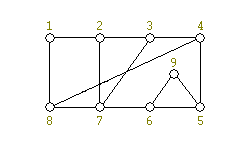
\includegraphics[width=8cm]{Term_2/Source/images/5_gamma_1.png}
\end{center}
\end{frame}

\begin{frame}[fragile]{Гамма-алгоритм}
 \textbf{Инициализация.} Находим любой простой цикл. 
 
 Получаем две грани: $\Gamma_1$ — внешнюю и $\Gamma_2$ — внутреннюю. Обозначим выбранный цикл как $G^{plane}$. 
\begin{center}
    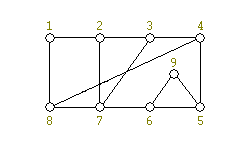
\includegraphics[width=6cm]{Term_2/Source/images/5_gamma_1.png}
    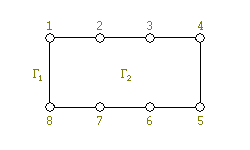
\includegraphics[width=6cm]{Term_2/Source/images/5_gamma_2.png}
\end{center}
\end{frame}

\begin{frame}[fragile]{Гамма-алгоритм}
\textbf{Шаг алгоритма.} Строим множество сегментов. Каждый сегмент S относительно $G^{plane}$ представляет собой одно из двух:
            \begin{itemize}
                \item ребро, оба конца которого принадлежат $G^{plane}$, но само не принадлежит $G^{plane}$;
                \item связную компоненту графа G – $G^{plane}$, дополненную всеми ребрами графа G, т.ч. один из концов принадлежит G – $G^{plane}$, а второй $G^{plane}$
            \end{itemize}
Те вершины, которые одновременно принадлежат $G^{plane}$ и какому-то сегменту, назовем контактными. Сегменты и вершины изображены на слайде справа. Контактные вершины обведены в квадрат.
\begin{center}
    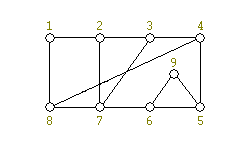
\includegraphics[width=4cm]{Term_2/Source/images/5_gamma_1.png}
    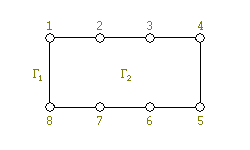
\includegraphics[width=4cm]{Term_2/Source/images/5_gamma_2.png}
    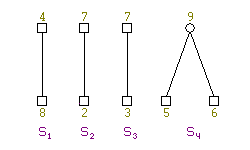
\includegraphics[width=4cm]{Term_2/Source/images/5_gamma_3.png}
\end{center}
\end{frame}

\begin{frame}[fragile]{Гамма-алгоритм}
\textbf{Утверждение.}\\
В каждом сегменте не менее 2 контактных вершин\\
Если бы 0, то несвязный граф\\
Если бы 1, то мост\\
Значит, в любом сегменте есть цепь между любой парой контактных вершин
\end{frame}

\begin{frame}[fragile]{Гамма-алгоритм}
Пока для любого i: $S_i \in {\Gamma_1, \Gamma_2}, |\Gamma(S_i)| = 2$. Поэтому возьмем первый по номеру сегмент $S_i$ и в нем первую попавшеюся цепь \{4, 8\}; вставим эту цепь в грань $\Gamma_2$. Получим увеличенную часть $G^{plane}$ и уменьшенную систему сегментов
\begin{center}
    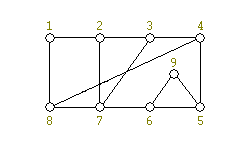
\includegraphics[width=5cm]{Term_2/Source/images/5_gamma_1.png}
    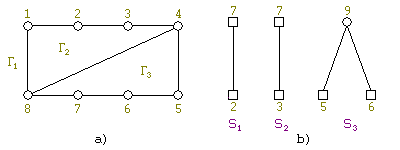
\includegraphics[width=5cm]{Term_2/Source/images/5_gamma_4.png}
\end{center}
\end{frame}

\begin{frame}[fragile]{Гамма-алгоритм}
Определим, какие грани вмещают новые сегменты. Теперь сегменты $S_1$ и $S_2$ вмещаются только в одну грань $\Gamma_1$, в то время, как сегмент $S_3$ вмещается в две грани $\Gamma_1$ и $\Gamma_3$. Поэтому берем $S_1$. Возьмем в нем цепь между контактными вершинами, например, \{2, 7\}, и уложим ее в $\Gamma_1$. Получим увеличенную часть $G^{plane}$ и уменьшенную систему сегментов 
\begin{center}
    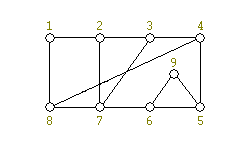
\includegraphics[width=4cm]{Term_2/Source/images/5_gamma_1.png}
    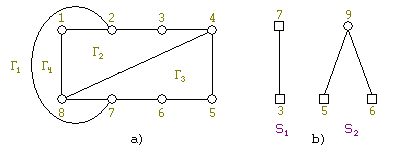
\includegraphics[width=7cm]{Term_2/Source/images/5_gamma_5.png}
\end{center}
\end{frame}

\begin{frame}[fragile]{Гамма-алгоритм}
Продолжая таким образом, в итоге получим плоскую укладку графа G
\begin{center}
    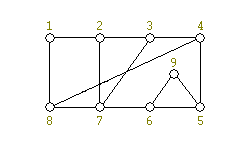
\includegraphics[width=5cm]{Term_2/Source/images/5_gamma_1.png}
    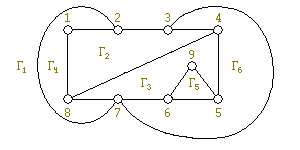
\includegraphics[width=5cm]{Term_2/Source/images/5_gamma_6.png}
\end{center}
\end{frame}

\appendix

\section<presentation>*{\appendixname}
\subsection<presentation>*{Useful links}

\end{document}


